% This example is a LaTeX document showing how to use the lmproj class to
% write your report. The chapter headings are by no means prescriptive. Instead
% use an appropriate report structure for your project as you see fit.
% Use pdflatex and bibtex to process the file, creating a PDF file as output 
% (there is no need to use dvips when using pdflatex).

% Modified 

\documentclass{lmproj}
\usepackage{amsmath}
\usepackage{listings}
\begin{document}
\title{Large-Scale Learning: Query-driven Machine Learning over Distributed Data}
\author{Kurt Portelli \\
        Natascha Harth \\
        Ruben Giaquinta \\
        Xu Zhang \\
        Monica Gandhi}
\date{1 December 2015}
\maketitle
\begin{abstract}
We study a novel solution to executing aggregation queries more specifically AVERAGE queries over large scale-data. We investigate cases where the owners restrict data access such that only aggregation operators can be used. It can also be extended to scenarios where access to the data is limited due to cost or slowness. Using distance-based queries with aggregation operators we are able to gain insight on how to best cluster the underlying data. The useful information are the results derived from the aggregation queries which are then clustered based on the distance based queries allowing us to then be able to predict the results of new and unseen queries. We study this approach which is called query-driven machine learning and evaluate its performance.

\end{abstract}
\educationalconsent
\tableofcontents
%==============================================================================
\chapter{Introduction}
\label{intro}
With the enormous improvements in performance and price in both data storage devices and network infrastructure it is now very cheap to store data. Since such large amounts of data is now accessible this has created a need and opportunity for machine learning algorithms.\cite{LargeScaleOnlineLearning} The challenge nowadays is not to store large amounts of data but to make it as accessible as possible. It is very difficult to query these datasets and return results interactively. According to L.Bottou and Y.Le Cunn\cite{LargeScaleOnlineLearning} these technological improvements have outran the exponential evolution of computing power. Thus, we must rely more on learning algorithms to process these large amounts of data with comparatively less computing power. These algorithms are typically split into online and batch. Online algorithms quickly process large datasets by adjusting their parameters as fresh data is inputted. On the other hand batch algorithms keep iterating over the dataset to achieve the optimum solution. It is then argued that online outperform batch algorithms due to the fact they do not iterate over a dataset.\cite{LargeScaleOnlineLearning}

In this work we are going to assume we are dealing with datasets which we don't have access to. In a real world scenario this can occur for a variety of reasons. It might be that the dataset is just too large to go through it, or the the third party REST API service that is being used has a cost for each query that is made. Another requirement might be that this third party company does not allow a copy of their data to be held. Thus, batch algorithms won't be able to iterate through the whole dataset or it might be too costly to do so. 

We will be investigating the use of online clustering in machine learning with the aim to finally be able to predict the results of queries without running them on the dataset. We will also be using a query driven approach \cite{LearningDNN} which will allow us to only quantize the important areas inside the data space. This approach creates various subspaces of interest  which are determined by a focal point in space and radius. The AVERAGE aggregation operator will be studied to gain an insight on how best to cluster the underlying dataset. The goal is to use the results of the queries issued to cluster the underlying data. Online clustering is used because these results represent a stream of infinite data which the clustering can learn over time.

Before going in detail about the training set generation, learning and prediction process, in the following section traditional algorithms and related work are going to be discussed to better compare our achievements.

%==============================================================================
\chapter{Related work}
\label{relatedWork}
The general approach in learning a large multi-dimensional dataset is to investigate the dataset as a whole and estimate the probability density function. G.Cormode et al. in \cite{Synopses} describes the well established techniques used in aggregate query processing. They mention histograms, self tuning histograms, sketches, sampling and wavelets. As C.Anagnostopoulos and P.Triantafillou argue in \cite{learningCount} these techniques assume that they have access to the actual data set, thus can store and preserve the statistical model created. For example to be kept up to date, histograms need to scan all the data. On the other hand Self-tuning histograms execute additional queries to adjust the statistical model accordingly.

GENHIST\cite{Genhist} is one of the variations of histograms with the same target, to find an approximate density function using a grid. GENHIST achieves this by iteratively split the dataset into regular grids and find the dense areas. In each iteration the density of each bucket with the surrounding buckets is smoothed. The innovation behind this is that in each iteration buckets may overlap thus, revealing new information and a more accurate density function. In each iteration buckets are removed which effect the number of iterations, for example a high value can result in losing important detail. Although the number of iterations is a constant number which depends on the parameters given this still scales directly with the size of the dataset. Each iteration involves doing one pass over the data and since the number of iterations is constant, the running time of the algorithm is constant.\cite{Genhist}

As the dataset changes over time the GENHIST algorithm has to be run again to update the probability density function. As the dataset increases in size, traditional histograms such as GENHIST fail to scale well due to the fact that they regularly need to be rebuilt to update the statistical model creating a substantial overhead. It is then noted that the statistical models created by histograms only consider the data distribution without taking into consideration the query pattern of users.\cite{learningCount} Thus, this is not suitable for what we want to achieve, as we are interested in a constructing a model that relies on the query distribution and data distribution. Self-tuning histograms (STH) were proposed to address this by using the cardinality of a query's result to adjust the statistical model. STH still have a fundamental limitation which is the necessity of reading all the dataset because it needs to calculate the probability density function. The use of wavelets, sketches and sampling are also discussed in \cite{learningCount} with the conclusion that they are not viable since they need to access the raw data to create and maintain their structures.

In \cite{learningCount} the query driven approach is discussed in detail and compared to the techniques mentioned above. The query driven approach is very useful in the scenario where one does not have access to the data or it is very costly to access the data (maybe due to size, cost, location). The idea behind this approach is that a training set containing a list of queries with their corresponding output is given. After learning this training set the algorithm should be able to predict the output without running the query. Although the training set is extracted from the dataset it is independent from the size of the dataset. Thus the size of the dataset will not impact the performance and the quality of the prediction fully depends on the training set and prediction algorithm used.

C.Anagnostopoulos and P.Triantafillou\cite{learningCount} discuss how this training set can be manipulated to allow the algorithm to predict results from queries as fast and accurate as possible. It is accepted that new queries might not be found in the training set thus a way to identify how close a query is to another is to use euclidean distance. One can go through all the training set, find the closest training query and then return the result of that query. This solution would increase linearly on the size of the training set. But, some queries might be redundant since they are very close to other existing queries while others might be significantly more important since they define another whole separate user interest. This shows the importance to extract information from the query space and be able to find the interest areas. Thus, the solution would be to cluster similar queries into a smaller set of representative queries called \textit{L}.

To arrive at the prediction stage each representative query is assigned a representative result. The representative results are continuously updated while learning and moved around the data space depending on the training set. If the training space is large enough the representative queries and results should converge to represent what is actually inside the raw data. The clear advantage is that the size of \textit{L} is smaller than the size of the training set which in turn is smaller than the raw data.\cite{learningCount}

Learning can easily be stopped and continued without the need to start from scratch. This approach makes prediction very fast since each new query is associated with a closest representative query and the representative result given. In case the actual result is known the prediction error can be calculated by checking the difference between the actual and predicted result.\cite{learningCount}

%==============================================================================
\chapter{Design \& Implementation}
\label{design}

\section{Clustering}
The problem of cluster analysis consists in grouping a set of objects, the data set, in clusters (groups), according to similar features. Similarity among objects is mainly related to the concept of Euclidean distance. In this section some clustering algorithms will be presented.

\subsection{Nearest Neighbour - Average Data}
The Nearest Neighbour algorithm is one of the simplest methods for classification. The algorithm, given a finite set of d-dimensional vectors $X=\{x^t\}_{t=1}^{N}$, each with a class label, and a defined constant $k$, partitions the space classifying each point $x \in X$ as the majority class between the $k$ nearest neighbors. In order to find the $k$ nearest neighbors, the function calculates for each $x \in X$ the Euclidean distance between $x$ and $x'$, $\forall x' \in X$.
\subsection{Offline K-Means}
\subsubsection{The Algorithm}
Batch K-Means is the oldest and most simple clustering method; it is however very efficient. The algorithm, given a finite data set of d-dimensional vectors $X=\{x^t\}_{t=1}^{N}$ and $k$ \textit{centroids}, or \textit{codebook vectors}, $m_j,j=1,...,k$, partitions the data set into $k$ clusters in order to minimize the so called total \textit{reconstruction error}, defined as follows:
\begin{equation}
E(\{m_i\}^k_{i=1}|X)=\underset{t}{\sum}\underset{i}{\sum}b_i^t
\end{equation}
where
\begin{equation}
b_i^t=
\begin{cases}
1 & if \parallel x^t -m_i \parallel = min_j \parallel x^t - m_j \parallel \\
0 & otherwise.
\end{cases}
\end{equation}
Therefore, $x^t$ is represented by $m_i$ with an error proportional to the Euclidean distance $\parallel x^t - m_j \parallel$. The procedure starts initializing $m_i$ randomly; at each iteration $b_i^t$ is calculated for all $x^t$ and $m_i$ is updated according to the following rule:
\begin{equation}
m_i=\dfrac{\sum_t b_i^t x^t}{\sum_t b_i^t}.
\end{equation}
The algorithm terminates if any of the \textit{codebook vectors} $m_i$ hasn't been changed during the update step. Upon termination the function returns the \textit{codebook verctors}\cite{Clustering}.

\subsubsection{Implementation}
The Batch K-Means was implemented in Java. The Cluster class has two objects, an \textit{ArrayList} of \textit{points} representing all the points belonging to the cluster, and a \textit{centroid}, the \textit{codebook vector}.
The update function searches for the nearest \textit{codebook vector}.
\lstinputlisting[language=Java, basicstyle=\tiny, firstline=58,lastline=76]{OfflineKmeansN.java}
At a later stage the method applies the update rule for each of the \textit{codebook vectors}, counting the number of updated \textit{centroids}.
\lstinputlisting[language=Java, basicstyle=\tiny, firstline=78,lastline=120]{OfflineKmeansN.java}
The function terminates if the value of the variable counting the number of modified centroids is equal to the number of clusters $counter == Clusters.size()$.


\subsection{Online K-Means}
\subsubsection{The Algorithm}
The Batch K-Means cannot, or at least not efficiently, deal with huge data sets. Storing a vast amount of data in internal memory can be a serious issue. In order to avoid this problem, Online K-Means does not store input data. Therefore, the algorithm initialize $k$ random \textit{codebook vectors} $m_j,j=1,...,k$ from the training set $X$. For all $x^t \in X$, randomly chosen, the update function computes:  
\begin{equation}
i \longleftarrow arg min_j \parallel x^t - m_j \parallel
\end{equation}
\begin{equation}
m_i \longleftarrow m_i + \eta (x^t - m_i)
\end{equation}
until $m_i$ converge \cite{Clustering}.

\subsubsection{Implementation}
The Online K-means was implemented in Java as well. The update method is presented below:
\lstinputlisting[language=Java, basicstyle=\tiny, firstline=23,lastline=40]{OnlineKmeans.java}
The first $k$ input stream points are added as centroids; at a later stage, the \textit{classify} function is called in order to search for the nearest centroid and update it accordingly.
The \textit{moveCentroid} method is implemented according to the rule: 
\begin{equation}
m_i \longleftarrow m_i + \eta (x^t - m_i).
\end{equation}
The class Tools defines a set of multi dimensional operations like the Euclidean distance, addition, subtraction and multiplication, and finally a method to find the minimum value. 
\lstinputlisting[language=Java, basicstyle=\tiny, firstline=11,lastline=31]{Tools.java}

\subsection{ART}
\subsubsection{The Algorithm}
Adaptive Resonance Theory (ART) is a competitive learning algorithm used in neural networks. The algorithm follows an incremental approach, initializing just one centroid and adding other centroids as needed. ART does not require the number of clusters to be specified, instead it requires a \textit{vigilance} in order to create new centroids.

In ART, initially the first input point is chosen as the centroid for the first cluster. When the Euclidean distance between the data point and its nearest centroid is less than the vigilance, then the update is calculated as in Online K-Means. However, if the distance is greater than the vigilance, then a new cluster is created with that point as a centroid.

For the data set $X = \left\{ {x^{t}}\right\}_{t=1}^N$, the following equations are performed for each update:
\begin{equation}
b_{i} = \parallel{m_{i}} - x^{t}\parallel  = \min_{l=1}^k \parallel  m_{l} - x^{t}∥
\end{equation}
 
\begin{equation}
\begin{cases}
m_{k+1}\leftarrow x^{t} & if b_{i}>\rho
\\\triangle{m_{i}}=\eta\left(x^{t} - m_{i}\right) & otherwise
\end{cases}
\end{equation}

$m_{i}$ is the initial cluster center, $\rho$ is the vigilance value specified by the user and $b_{i}$ is the minimum distance of the point to its nearest cluster center \cite{Clustering}. 
 
\subsubsection{Implementation}
The ART algorithm has been implemented in Java and includes three classes: \textit{ART}, \textit{Application} and \textit{Tools}. The Application class requires the text file containing the data points, the vigilance value and the alpha learning value as input while the \textit{Tools} class contains a set of multidimensional operations.

The ART class implements the \textit{update} function as per the equations 3.7 and 3.8 for each input data point. The variable \textit{row} is the user input vigilance value and \textit{point} is the next incoming data point. \textit{Tools.distance(point, centroids.get(nearestCentroid))} gives the minimum distance of the point to its nearest cluster center.

\lstinputlisting[language=Java, basicstyle=\tiny, firstline=21,lastline=39]{ART.java}

If the distance between the point and the nearest centroid is less than the vigilance value, the method invokes the \textit{moveCentroid} function which adds the point to the cluster and updates the centroid.

\lstinputlisting[language=Java, basicstyle=\tiny, firstline=40,lastline=45]{ART.java}

The output is obtained in two different text files, one containing all the centroids of the cluster and the other file containing the cluster ids of each data point.

\subsection{Silhouette}
\subsubsection{The Algorithm}
Silhouette is an evaluation method used to determine how well a data point lies within its cluster. This method is used to validate the consistency and strength of a cluster. The Silhouette Coefficient of a data point, s(i) can be determined using the following formula:
\begin{equation}
s(i) = \frac{b(i) - a(i)}{max\left\{a(i), b(i)\right\}}
\end{equation}
which can also be expanded as,
\begin{equation}
s(i) = \begin{cases}
1-a(i)/b(i) & if a(i)<b(i)
\\0 & if a(i)=b(i)
\\b(i)/a(i) -1 & if a(i)>b(i)
\end{cases}
\end{equation}
where a(i) is the average distance from the $i^{th}$ point to the other points in the same cluster and b(i) is the minimum average distance from the $i^{th}$ point to points in a different cluster \cite{Rousseeuw}.

The values $s(i)$ of a silhouette coefficient usually ranges from $-1$ to $1$. If $s(i)$ is close to 1, it means that the point is in the right cluster. If $s(i)$ is close to zero, then the point lies near the decision boundary of two neighboring clusters. Otherwise, if $s(i)$ has negative values, it means that the point is in the wrong cluster.

The average silhouette values of all the points in the cluster is used to determine the quality of the clustering method used. Hence, the optimal number of clusters for an efficient clustering would be the number of clusters that gives the highest silhouette coefficient.
\subsubsection{Implementation}
The silhouette algorithm has been implemented in MATLAB using the function \textit{silhouette(X,clust,metric)} where X is the matrix of data points, \textit{clust} is the cluster \textit{ids} of each data point and metric is the inter-point distance function used. 

The variable \textit{data} is the path to the text file containing the data points while the variable \textit{kmeans} is the path to the text file containing their corresponding cluster numbers. The metric we used is the Euclidean distance between the points.

\lstinputlisting[language=Matlab, basicstyle=\tiny]{Silhouette.m}
The above program gives the mean Silhouette coefficient of the overall points in the cluster.

\section{Query Space Clustering}

The Online K-Means described at 3.1.3 provides an efficient approach to address huge data sets without accessing raw data. However, it is easily to notice that the input of Online K-Means (i.e., the output of queries) is randomly and uniformly chosen. This is obviously unreasonable. Thus, the challenge here is that how to generate an appropriate input for Online K-Means. Before exploring the specific solution, it is necessary to give a definition for query and explain the generation of a query. 

\subsection{Original Query Generation}

A query Q has two parts: the input of the query, which called query-point, X and the radius THETA, where X is a multidimensional vector from the real dataset and THETA is the ‘radius’ with a constant value. 

\begin{equation}
	q =[\vec{x},\theta] =[x_1,x_2,...,x_n,\theta] (n-dimension)
\end{equation}

For example, consider dealing with a dataset S with two-dimensional points. The query-point is X=[X1, X2]. In the Online K-Means mentioned before, the values of X1 and X2 are chosen uniformly and randomly from S. The next step is to scan ALL the data and gather all data points Z, for instance, Z = [Z1, Z2] such that the Euclidean distance between Z and the query-point X is less than THETA. Subsequently, record the average of all Z points that satisfy the criterion: less than THETA, and notate this as the output of a query. Finally, if there are M queries, repeat this process of query generation for M times and save all the output as the input for Online K-Means. 

\subsubsection{Implementation}
The original query generation was implemented in Java. The methods are shown below:

\lstinputlisting[language=Java, basicstyle=\tiny, firstline=49,lastline=60]{OriginalTools.java}

This function is used to generate a set of queries randomly with two parameters: int queryLimit (i.e., M queries) and int noOfAxis (i.e., the dimensions of points). r.nextFloat() will return the next uniformly distributed float value between 0.0 and 1.0 and then minus 0.5 simply because the range of dataset in this case is from -0.5 to 0.5.

\lstinputlisting[language=Java, basicstyle=\tiny, firstline=25,lastline=30]{OriginalTools.java}
\lstinputlisting[language=Java, basicstyle=\tiny, firstline=15,lastline=21]{OriginalTools.java}
The loop scan all dataset to find all points Z that the distance less than THETA and then search the center of Z. Tools.distance() can calculate the Euclidean distance between two points.
\lstinputlisting[language=Java, basicstyle=\tiny, firstline=33,lastline=47]{OriginalTools.java}
The idea here is that using a loop to count the sum of Z for each dimension and then compute the mean value for each dimension.

However, the original idea of query generation has two limitations. Firstly, as mentioned above, users is less likely to issue queries from the whole dataset uniformly and randomly. Another problem is that this method needs to scan whole dataset to find all the points that the distance less than THETA. It is likely to increase a heavy load and cost especially when addressing a large-scale dataset. Query Space Quantization (i.e., Query Space Clustering) is proposed to solve these problems. 

\subsection{Pre-define Data Subspaces by Interest Points}
To begin with, it is necessary to pre-define some data subspaces in order to simulate the areas of interest of a user. Assume that there are L = 10 subspaces in a 2-dimensional dataset. That is, the user normally issues queries from L data subspaces. More specifically, fix a data subspace, say subspace J, J = 1, ..., L. The subspace J is modelled through a Gaussian distribution of 2 dimensions, i.e., a mean value M1 for dimension X1 and a mean value M2 for dimension X2 are needed. Furthermore, for simplicity, assume that the variances V1 and V2 for dimensions X1 and X2 are the same and fixed, e.g., V1 = V2 = 0.01. 


\subsection{Select a Subspace and Generate a Query}
Secondly, assume that there is a need to generate N = 10000 queries from L = 10 subspaces. That is, a subspace J is firstly chosen from 1 to 10, each one with equal probability, i.e., J = Random(1,10). Then, from the J-th subspace, a query is generated as discussed above. Intuitively, 10000/10 = 1000 queries will be generated from each subspace J, J = 1...10. 

Next, to generate a query from the J-th subspace, it is necessary to set the center of query-points X = [X1, X2] and the THETA value is fixed, e.g., THETA = 0.1. The X1 is generated by the Gaussian with mean M1 and variance V1. The same holds true for X2. That is, X1 = Random.Gaussian(M1,V1) and X2 = Random.Gaussian(M2,V2). Hence, the query with the center of query-points X = [X1, X2] and radius THETA is located within the J-th subspace, i.e., in a disc of center [M1, M2].

\subsubsection{Implementation}

\begin{minipage}[b]{0.5\linewidth}
-0.4,0.2,0.01

-0.3,-0.3,0.01

-0.4,0.4,0.01

0.2,0.3,0.01

-0.1,-0.1,0.01

0.1,-0.3,0.01

-0.25,0.25,0.01

0.4,0.1,0.01

0,0,0.01

0.2,-0.2,0.01

\end{minipage}
\hfill
\begin{minipage}[b]{0.5\linewidth}
	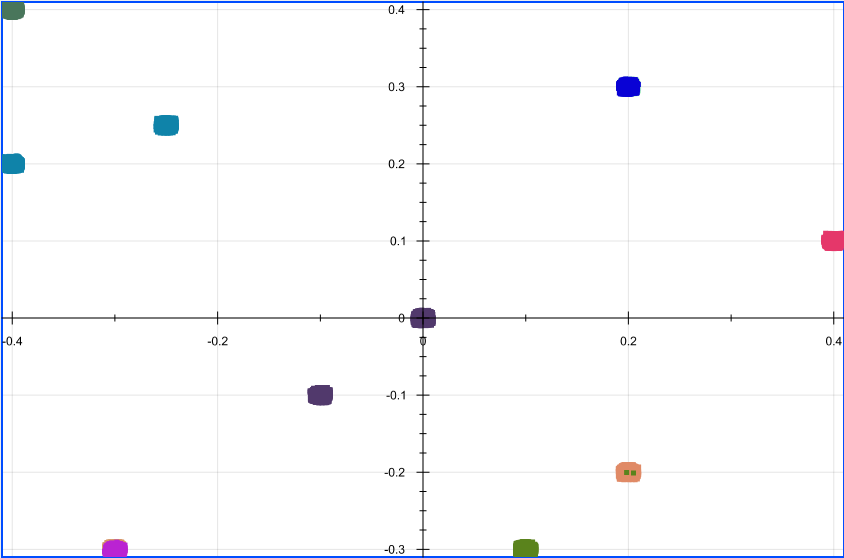
\includegraphics[height=10\baselineskip]{L.png}
\end{minipage}

The left side is a typical file format of J, i.e., M1,M2,V1(V2). The picture is the visualization for this subspace.

The generation of points, which follow Gaussian distribution, was implemented in Java. The function is presented below:
\lstinputlisting[language=Java, basicstyle=\tiny, firstline=102,lastline=117]{Tools.java}
\lstinputlisting[language=Java, basicstyle=\tiny, firstline=10,lastline=14]{Tools.java}
There are two parameters. Float[] point represents the center [M1, M2]. Float width means the variance V1=V2=0.01. r.nextGaussian() returns the next Gaussian distributed double value with mean 0.0 and standard deviation 1.0. And then multiplying by (width/3) enables about 99.7\% of a population will be within the range (-0.01, 0.01). Finally, moving this number towards the center X by adding the mean value M1 or M2. 




\subsection{Online Quantization}
Finally, the concept here is to address overload for large-scale dataset by avoiding storing all the queries, scanning all dataset and then calling a batch K-means. In the reality where users issuing queries, it is essential to quantize them ONLINE. That is to incrementally generate queries and then injecting each one to the incremental K-means algorithm, for quantizing the query vectors. Obviously, if K = L then after a lot of queries, you will see that ALL the K means vectors will be the vectors with dimensions (M1[J],M2[J]) since, naturally, the K-means algorithm learn the query distribution, which in our case in a L-modal Gaussian distribution, i.e., L = 10 Gaussian bells.

\subsubsection{Implementation}

\lstinputlisting[language=Java, basicstyle=\tiny, firstline=123,lastline=129]{QueryClustering.java}
queryLimit in this part of loop means represents M queries. For each query, inject it to online K-Means and then get centroid. 

Evaluation the similarity of the queires:

Plot the K means over the space to check their positions to check the distance to the positions of the M1[J], M2[J], J = 1, ..., L. The distance between two queries is the Euclidean distance of their centers and their THETA values, i.e., Q1 = [X1, X2, THETA] and Q2 = [X1, X2, THETA]. 
\begin{equation}
DISTANCE (Q1, Q2) = (Q1.X1-Q2.X1)^2+(Q1.X2-Q2.X2)^2+(Q1.THETA -Q2.THETA)^2.
\end{equation} 
In this case, THETA is the same for all queries. This distance quantified the similarity of the queries.

Further work:
For each subspace, it is chosen from 1 to 10 with equal probability. It is a rare situation in the reality. Some probability theories and predictive methods could be involved in, such as Bayesian inference. On the other hand, for each subspace, it is modeled by Gaussian distribution. Although it is the most common distribution, some other models, such as linear regression, could also be considered. Combining with some inference theories, this can be more specific. 

\clearpage
\section{Prediction}
Within the prediction sections 3.1 and 3.2 with their described techniques are join up with each other but only under consideration of two dimensional data. The intent outcome of the prediction is to find the average data point of a query without scan through the behind dataset. 

To achieve this a trainings set is needed to learn the machine algorithm to finally test with another dataset how good this learning was. The goodness of this machine learning algorithm, the exact evaluation, will be explained in chapter 4. In this section the implementation of creating he training and test set, learning the algorithm and predict the outcome from a query input will be described in the following subsections. Each subsection represents a standalone application which can be run through the generated batch file with modifying the depending input variables. 

\subsection{Mapping query and output data}

The fundamental for a successful prediction is to create a training set that is mapping the query that was generated through the actual output, the average data point.

A query is define in equation 3.7 with a point \textit{x} for each dimension and theta, the radius a constant in our work.  
\begin{equation}
q=[x_1,x_2,\theta] =[\vec{x},\theta]
\end{equation}
For each query a output will be generate that contains the average data point of all data points from the real dataset inside the define radius theta. Therefore the output of a query is define as:
\begin{equation}
\bar{x}=[\bar{x_1},\bar{x_2}]=\frac{1}{n}\sum \vec{x_i}:\parallel \vec{x}-\vec{x_i}\parallel \leq \theta
\end{equation}
Figure \ref{fig:Query} visualise this technique by showing a two dimensional dataset with a query as blue and the radius theta further the actual dataset points as black and the average data point as red circle.
 \begin{figure}[ht]
	\centering
	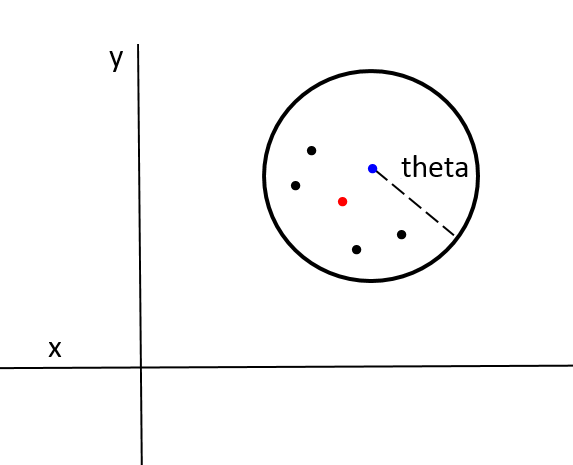
\includegraphics[width=0.6\linewidth]{Query.PNG}
	\caption[Query]{Query and average data point creation}
	\label{fig:Query}
\end{figure}

The exact approach and implementation will be found in section 3.2.1.. With our definition of query and the related output for each query we can define our training set as:
\begin{equation}
Trainingsset=[q,\bar{x}]
\end{equation}

\subsubsection{Implementation}

The implementation of mapping a query and the average data point with Java is done with the following code extract of the java class QueryGE:

\lstinputlisting[language=Java, basicstyle=\tiny, firstline=42,lastline=58]{QueryGE.java}

Inside the \textit{for} loop a random query will be generate with the method \textit{generateQuery()} either inside the ranges of define subspace explained in section 3.X or if no subspace is define over the whole dataset. After a query was generated the average data point for this query will we located through the method \textit{generateAverageDataFromQuery()}. Both query and average data point are stored in a float array. The final coordinates of the query and the average point will be than written into a semicolon separated file using \textit{BufferedWriter}.

The whole application \textit{TrainingSetAppliction} can be run by giving a dataset, theta, a number of queries and a file with subspaces the user is interested in.
After train the machine learning algorithm a test set is needed in the same structure than the training set therefore this application can be used also for creating the test set. 


\subsection{Learning algorithm}

Learning from the previously generated training set we can use the online k-means algorithm. This concept was explained in section 3.1.1 with the implementation in this project. 
A short summary of the key facts: the online k-means sets the first k points as cluster centroids and moves the nearest centroid for the next point in its direction with a fix alpha. 
The following paragraph will explain how we connected the online k-means approach with our training set and how we created our set for the prediction.

To find the centroid of all queries we give one by one to the online kmeans algorithm. At the same time another instant of the online k-means gets the related average point. This is implemented in our java class \textit{LearningApplication} in row 64-65, see following code extract:

\lstinputlisting[language=Java, basicstyle=\tiny, firstline=64,lastline=65]{LearningApplication.java}

Important is that the connection between cluster of query and average point is still established. Wherefore we store the cluster id of our average data on the same position than the query cluster id. This can be seen in this code extract:
\lstinputlisting[language=Java, basicstyle=\tiny, firstline=66,lastline=66]{LearningApplication.java}

With this system we having after running the online k-means through the whole training set a list of cluster id of our average data on the position of the query cluster id. As a result we can write the centroid of our queries defined in equation 3.10 with the related centroid of the average data defined in equation 3.11 in a file by using \textit{BufferedWriter}. See posterior code detail:
\lstinputlisting[language=Java, basicstyle=\tiny, firstline=70,lastline=82]{LearningApplication.java}

Therefore our prediction set will be containing the centroid of our queries w[j] and the correspondent centroid of the average data u[j], see the following notations for definition.
\begin{equation}
w[j]= online\,k-means\,centroids\,for\,q
\end{equation}
\begin{equation}
u[j]= online\,k-means\,centroids\,for\,\bar{x}
\end{equation}
\begin{equation}
Prediction\,set=[w[j],u[j]]
\end{equation}

\subsection{Prediction algorithm}

In the last application our previous generated prediction and a new test set will be used to predict for each query inside the test set a average data point without scanning through the dataset.

To predict the average point we try to find for each query the alike query-centroid. This can be done by using the nearest neighbour algorithm. It is calculation the euclidean distance between a point and a list of points and gives you for this point the nearest. For more details and the exact implementation go to section 3.1.1. After we found the nearest query centroid for this query we can find the correspondent average data centroid and declare it as our predicted \textit{xbar}.  

This logic can be found inside the java class \textit{PredictionApplication} between row 66 and 69. 
\lstinputlisting[language=Java, basicstyle=\tiny, firstline=66,lastline=69]{PredictionApplication.java}

These rows calling the method \textit{classify()}, which is explained in section 3.1 with more detail. This method is having as input the list of centroids and the new query of the test set, the returning is the nearest centroid of queries for the input query. Afterwards the centroid of the average data can be easily found and is marked as our predicted \textit{xbar}.

To evaluate the goodness of our predicted \textit{xbar}, we can define an error value for each query. This error value is define in 3.13 as the euclidean distance between the predicted \textit{xbar}, our centroid, and the actual \textit{xbar}.

\begin{equation}
	\epsilon_i = \parallel \bar{x} - u[j] \parallel 
\end{equation}

Implemented in java it can be found in the \textit{PredictionApplication} java class in row 71:

\lstinputlisting[language=Java, basicstyle=\tiny, firstline=71,lastline=74]{PredictionApplication.java}

For a summary evaluation it is possible to calculate the mean error over the tet set by sum each error and divide it through the number of queries in the test set. The mean error is define in equation 3.14.

\begin{equation}
Mean\,Error= \frac{\sum\epsilon_i}{i}
\end{equation}

The following code rows explain the implementation in our project using java:

\lstinputlisting[language=Java, basicstyle=\tiny, firstline=79,lastline=79]{PredictionApplication.java}

Further evaluation can be done by reading the result file that will be produced through the prediction. This file contains for each query the predicted average data point and the actual also the error value. At the end of this file the mean error is displayed. Inside the java code the following line is writing the outout by using \textit{BufferedWritter}:

\lstinputlisting[language=Java, basicstyle=\tiny, firstline=75,lastline=75]{PredictionApplication.java}

%==============================================================================
\chapter{Evaluation}
\section{Silhouette}
For a better understanding of the impact of vigilance and theta values in ART, we tested the algorithm with different values for both variables, evaluating the average clustering results with silhouette. As we already mentioned before, silhouette algorithm computes the average result for all the clusters evaluations. It is possible to notice that the performance is proportional to theta; however, for greater vigilance values the difference in performance as theta varies becomes more negligible.
The number of radius queries generated and executed over the original data space in order to test ART is $200.000$.

 \begin{figure}[ht]
	\centering
	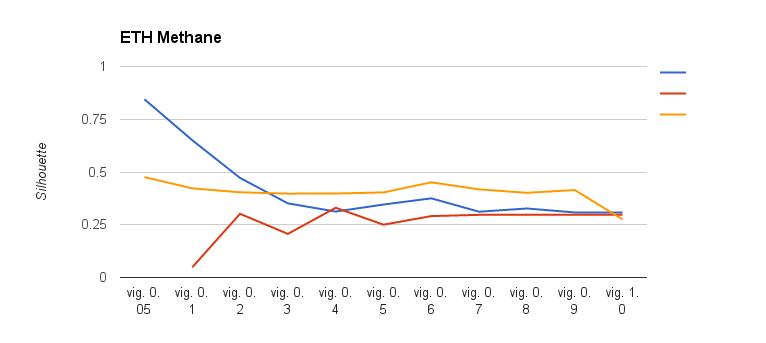
\includegraphics[width=1.1\linewidth]{thetavigilance.png}
    \caption[ARTevaluation]{The impact of Theta and vigilance in ART}
\end{figure}

Batch and Online K-Means were tested as well with different values of $k$ ($50,150,400$) and $theta$ ($0.05,0.2$) for the queries. For K-Means functions the number of radius queries is $100.000$.



\section{Error}
%==============================================================================
\chapter{Conclusion}
We have have studied a novel solution to the problem of predictive analysis over distributed data. This query driven solution is able to abstract query similarity and cluster the underlying data. The query clusters are associated with their related underlying data. The results of new queries are predicted by using the most similar query cluster. We evaluated this solution by using an evaluation data set to confirm that the predicted results are similar to the actual results. The significance of this study lies on the fact that it can predict results with restricted access to the dataset. This is due to the how the online learning mechanism is implemented, the prediction and learning steps are independent to the dataset, thus offering a scale-out and decentralized solution. 

%==============================================================================
\section{Contributions}


%==============================================================================
\bibliographystyle{plain}
\bibliography{example.bib}

\end{document}

